% \appendix

\chapter{Ablation studies}

\section{Stratified Sampling}

When sampling snippets of specified length from the dataset, we use a stratified sampling approach.
We do this to avoid draws where a snippet is repeatedly sampled from a single region of a trial.
Such an imbalance could lead to overfitting to a portion of the dataset and, generally, to treating various regions disproportionately.
We study the effect of this approach and find that it may matter less than we anticipated.

Recall that the stratified approach means sampling in \( n_{\text{strata}} \) consecutive turns from \( n_{\text{strata}} \) disjoint regions of the sampled dataset.
The parameter \( n_{\text{strata}} \) controls the granularity or the number of disjoint regions summing up to the full trial length.
We perform an experiment where we always sample 100 times from each trial, but vary the number of strata \( n_{\text{strata}} \).
We test on the task of song identification in the MUSIN-G dataset.
The results are shown in the graph below and, at most, seem to suggest a detrimental effect of such sampling when used with the XGBoost model. 
The effect seems small enough that we can follow the intuition behind the stratified approach and use it regardless.

\begin{figure}[H]
  \centering
  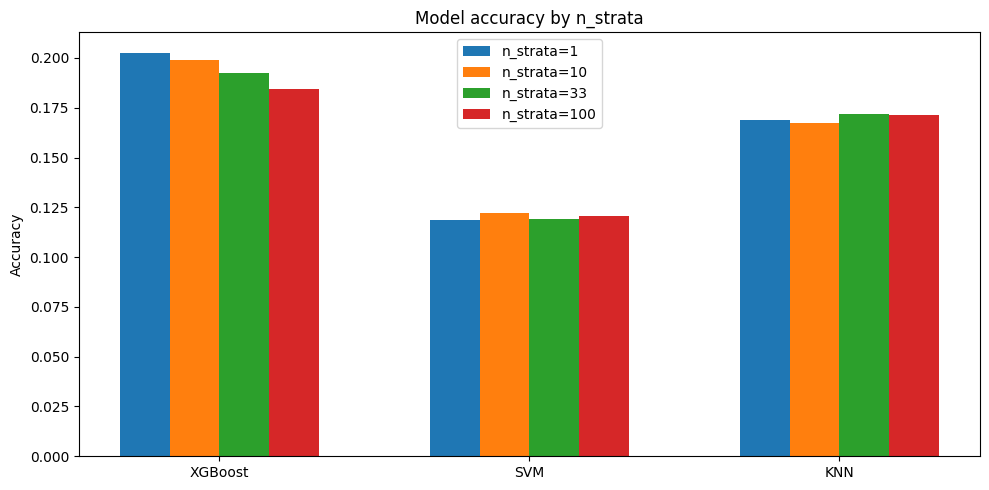
\includegraphics[width=0.8\linewidth]{imgs/stratified_uselesness.png}
  \caption{Effect of stratified sampling on classification accuracy.}
  \label{fig:stratified-sampling-ablation}
\end{figure}


\section{ICA}

In the preprocessing of the EEG data, we use ICA as a dimensionality reduction transform on the EEG signal.
ICA finds a linear transform of the EEG signal into so-called independent components, which are ordered by importance.
Similar to the use of PCA, we can drop the bottom components and reduce the number of channels in the EEG data.
We compare this use of ICA in preprocessing to picking a set of channels and dropping the rest.
The set of channels to be picked in this ``No ICA'' case is predefined and chosen based on proximity to auditory processing regions of the brain or a known relation to music processing.

\begin{figure}[H]
  \centering
  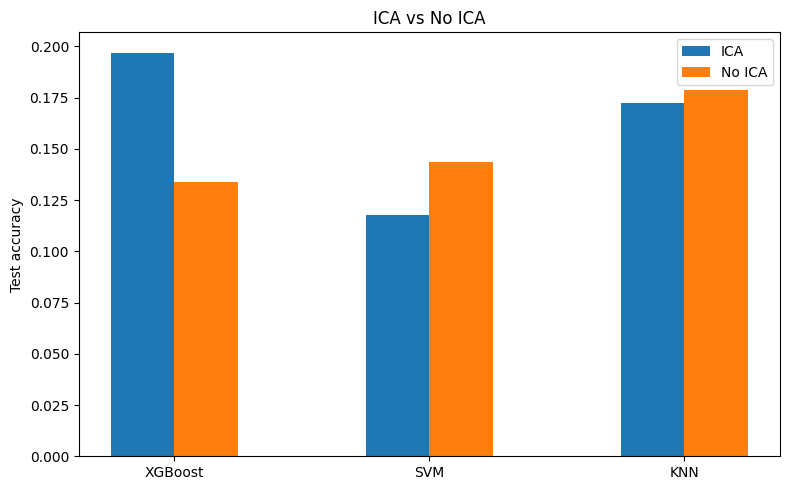
\includegraphics[width=0.8\linewidth]{imgs/ica_usefulness.png}
  \caption{Effect of ICA on classification accuracy.}
  \label{fig:ica-ablation}
\end{figure}

The results as tested on the task of song identification in the MUSIN-G dataset are inconclusive.

\section{Band power features}

For most tasks we employ band power feature analysis to the EEG signal. 
This is almost the last step of our preprocessing pipeline, only before normalization and sampling.
This processing step is crucial, as we are unable to train a model directly on the raw EEG signal.
We attempted song identification---the simplest task---and observed models difficulty to 
not only converge into a meaningful accuracy, but even to minimize the loss function in the first place.
Testing the non-deeplearning methods was omitted due to huge memory use and computation time.